%!TEX root = ../dissertation.tex


\chapter{Magneto-thermal transport}
\label{ch:magneto-thermal_transport}
\newthought{Extending thermal transport studies} of two-dimensional systems into high magnetic fields will facilitate a new wave of condensed matter experiments. Paired with electrical transport, thermal techniques are sensitive to inter-particle scattering~\cite{muller_collective_2008, crossno_observation_2016, lucas_transport_2016}, quantum criticality~\cite{sachdev_quantum_2011, muller_quantum-critical_2008}, chargeless excitation channels~\cite{wakeham_gross_2011, kane_thermal_1996, li_ballistic_2005, mccollum_spin-wave_1964, bid_observation_2010, inoue_proliferation_2014, venkatachalam_local_2012}, and can even be used to extract the entropy of a system through the Gibbs relations~\cite{kuntsevich_strongly_2015}. Furthermore, Johnson noise and Joule heating are particularly suited to magnetic experiments as, in the linear diffusive regime\footnote{The linear diffusive regime assumes cooling is dominated by Wiedemann-Franz like diffusion, the electrical conduction is sufficiently diffusive (not ballistic), and the temperature rise is small compared to the absolute temperature scale.}, the ratio of the Johnson noise temperature (section~\ref{section:TJN}) to the heating power $P$ is insensitive to the current profile or form of the conductivity tensor (section~\ref{section:beta}) while remaining quite sensitive to the ballistic, chiral nature of quantum Hall states.

The techniques and methods applied in this chapter are described in detail in chapters~\ref{ch:johnson_noise_thermometry} and \ref{ch:thermal_conductance_via_electrical_noise}.

\section{Generalized transport coefficients}
\newthought{In the presence of a magnetic field}, an electric field in a conductor can induce a current with a component perpendicular to the applied fields. In general, the transport coefficients ($\sigma$, $\alpha$, and $\bar\kappa$) take on a tensorial form ($\hat\sigma$, $\hat\alpha$, and $\hat{\bar\kappa}$) such that
\begin{equation}
\left( \begin{array}{c} \vec J  \\ \vec q \end{array}\right) =  \left( \begin{array}{cc} \hat\sigma   &\  \hat\alpha \\  T\hat\alpha   &\ \hat{\bar\kappa}  \end{array}\right)\left( \begin{array}{c}  \vec E \\  -\vec\nabla T  \end{array}\right)   \label{eq:m_transeq}
\end{equation}
For systems with two spatial dimensions (x, y) and a perpendicular magnetic field, the transport coefficient are $2\times 2$ matrices relating the local charge and heat current ($\vec J$ and $\vec q$, respectively) to the local electric field ($\vec E$) and temperature gradient ($\vec\nabla T$). The electrical conductivity, defined as the response of the charge current to an electric field with no thermal gradient, is simply given by $\hat\sigma$. However, the thermal conductivity ($\hat\kappa$) is not symmetrically defined as the response of heat current to an applied temperature gradient in the absence of an electric field but instead defined in the absence of a charge current. Thus,
\begin{equation}
\hat\kappa \equiv \hat{\bar\kappa}-T\hat\alpha\hat\sigma^{-1}\hat\alpha
\end{equation}
The form of the transport coefficients are constrained by a number of symmetries: The off diagonal elements of Eqn.~\ref{eq:m_transeq} are related due to Onsager reciprocity\footnote{Let $\hat\alpha$ and $\hat{\bar\alpha}$ be the two offdiagonal terms of eqn.~\ref{eq:m_transeq}. Time reversal symmetry and thus Onsager reciprocity demand ${\alpha_{ij}(B)=\bar\alpha{ji}(-B)}$. But rotational symmetry forces $\alpha$ to be antisymmetric and thus ${\alpha_{ij}(B)=-\bar\alpha{ij}(-B)=\bar\alpha{ij}(B)}$. Where the last step was done by rotating $\pi$ along an in plane axis.}~\cite{mazur_onsagers_1953, smrcka_transport_1977} and rotational symmetry requires all coefficients be antisymmetric --- i.e all coefficients can be written in the form:
\begin{equation}
\hat\sigma=\left( \begin{array}{cc} \sigma_{xx}  &\  \sigma_{xy} \\ -\sigma_{xy}  &\ \sigma_{xx} \end{array}\right)
\end{equation}

For a degenerate Fermi liquid, it has been shown theoretically~\cite{smrcka_transport_1977} and experimentally~\cite{zuev_thermoelectric_2009} that the thermal-electric coefficient $\hat\alpha$ is related to the electrical conductivity $\hat\sigma$, component by component, via the generalized Mott formula:
\begin{equation}\label{eq:Mott}
\hat\alpha = e\sL_0T~\frac{\mathrm{d}\hat\sigma}{\mathrm{d}\mu}
\end{equation}
where $\mu$ is the chemical potential and $\sL_0= \frac{1}{3}(\pi k_B/e)^2$ is the Sommerfeld value of the Lorenz number~\cite{sommerfeld_zur_1927}. However, in clean graphene samples inter-particle scattering breaks the assumptions used to derive Eqn.~\ref{eq:Mott} and violations of the Mott relation have been measured~\cite{ghahari_enhanced_2016}.
While a similar theoretical treatment~\cite{smrcka_transport_1977} has shown the validity of the generalized Wiedemann-Franz law 
\begin{equation}\label{eq:WF_gen}
\hat\kappa = \sL_0 T\hat\sigma,
\end{equation}
several detailed calculations have predicted violations in graphene near landau quantization~\cite{dora_magnetotransport_2007, long_quantum_2011, gusynin_magnetic_2005} and several more in the hydrodynamic regime~\cite{muller_quantum-critical_2008, muller_collective_2008}.

\section{Classical Hall Effect}
\newthought{In low magnetic field} or high carrier density, such that landau quantization does not significantly modify the density of states, the tensorial form of $\hat\sigma$ can be calculated under the assumptions of the classical Hall effect yielding:
\begin{align}
\sigma_{xx} &= \sigma_0~\frac{1}{1+\tan^2(\theta_H)} \nonumber\\
\sigma_{xy} &= \sigma_0~\frac{\tan(\theta_H)}{1+\tan^2(\theta_H)} \label{eq:hall_sigma}
\end{align}
where
\begin{equation}
\tan(\theta_H) = -\frac{\sigma_0}{e}~\frac{B}{n},
\end{equation}
$\sigma_0$ is the zero field conductivity, $n$ is the charge density, and $B$ is the perpendicular magnetic field strength. 
\begin{figure}
\centering
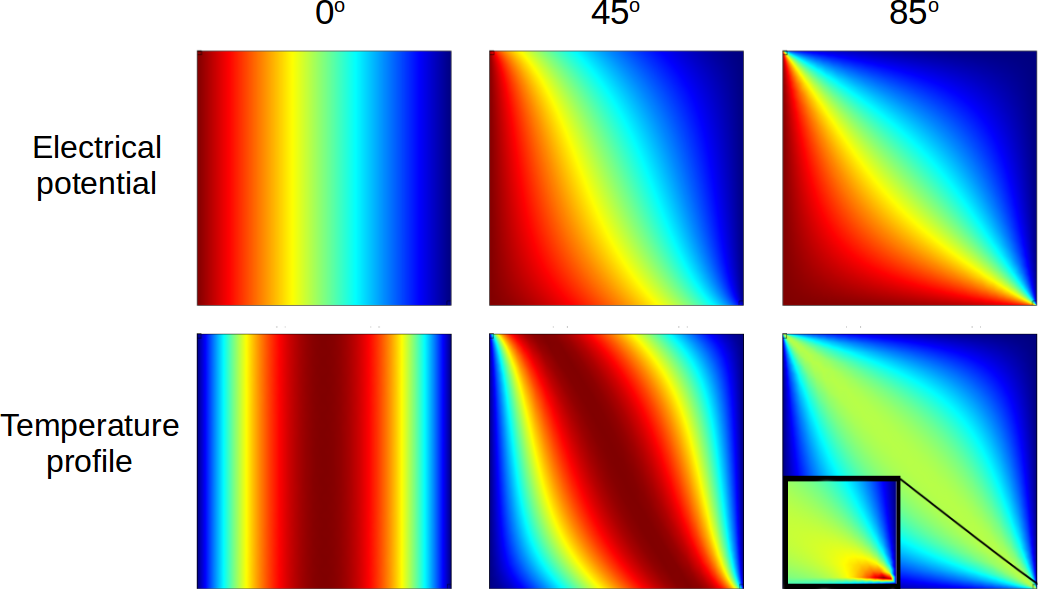
\includegraphics[width=120mm]{figures/magneto/Hall_profiles.png}
\caption{Normalized voltage (\textbf{upper}) and temperature (\textbf{lower}) profiles resulting from Joule heating a uniform, square conductor in the classical Hall regime for Hall angles $0^\circ$ (\textbf{left}), $45^\circ$ (\textbf{center}), and $85^\circ$ (\textbf{right}). The left and right sides of each profile correspond to electrical terminals with the the boundary conditions of constant voltage and temperature. For $\theta_h=0^\circ$ current flows uniformily from left to right and the temperature profile is parabolic as discussed in section~\ref{section:retangularDeviceJN}. As the Hall angle is increased, the current bends and the location of the peak temperature moves closer to the contacts. Near $90^\circ$, all of the dissipation occurs at the contacts resulting in the formation of hot spots. All plots are from finite element simulations~\cite{noauthor_comsol_2017}}
\label{fig:m_Hall_profiles}
\end{figure}

As the field strength increases, the changing conductivity tensor results in a changing current distribution, which, in turn, results in a changing Joule heating profile and steady state temperature distribution. Finite element simulations~\cite{noauthor_comsol_2017} illustrate how a magnetic field can affect the temperature and current profiles of a uniform, two-terminal conductor with the anisotropic $\hat\sigma$ and $\hat\kappa$ given by Eqn.~\ref{eq:hall_sigma} and Eqn.~\ref{eq:WF_gen}, as shown in Fig.~\ref{fig:m_Hall_profiles}. Boundary conditions are chosen to match a typical experiment where macroscopic electrical contacts serve as a thermal bath. In the absence of an external magnetic field, the current is uniform producing a parabolic temperature profile as discussed in section~\ref{section:retangularDeviceJN}. However, this simple calculation breaks down at finite field where current begins to bend, resulting in an anisotropic temperature profile. At large magnetic fields, where the Hall angle approaches $90^\circ$, nearly all the dissipation occurs at two points near the contacts resulting in the formation of hot spots. For a fixed Joule heating power, the spatial mean temperature of the sample goes to zero as Hall angle is increased and the hot spot size approaches a singularity; the power of Johnson noise measurements is that the measured Johnson noise temperature (section~\ref{section:TJN}), $T_{JN}$, naturally weights regions of higher local dissipation more such that as the dissipation approaches a singularity, so too does the spatial weighting function for $T_{JN}$ --- i.e. Johnson noise is sensitive to the temperature of the hot spots.

\section{Graphene characteristics}
\label{section:Giorgio}
\newthought{Monolayer graphene is mechanically exfoliated}, encapsulted with hexagonal boron nitride (hBN), and contacted along its one dimensional edge~\cite{wang_one-dimensional_2013} to form a square, two-terminal device ($4~\mu m\times4~\mu m$). These dimensions are chosen as a balance between the requirements that the device be longer than the electronic mean free path yet short enough that Wiedemann-Franz cooling dominates over electron-phonon cooling, as discussed in chapter~\ref{ch:thermal_conductance_via_electrical_noise}. Samples are fabricated on insulating sapphire substrates with a local top gate to electrostatically control carrier density as shown in Fig.~\ref{fig:m_Giorgio}. The gate capacitance is measured using the integer quantum Hall effect.
\begin{figure}
\centering
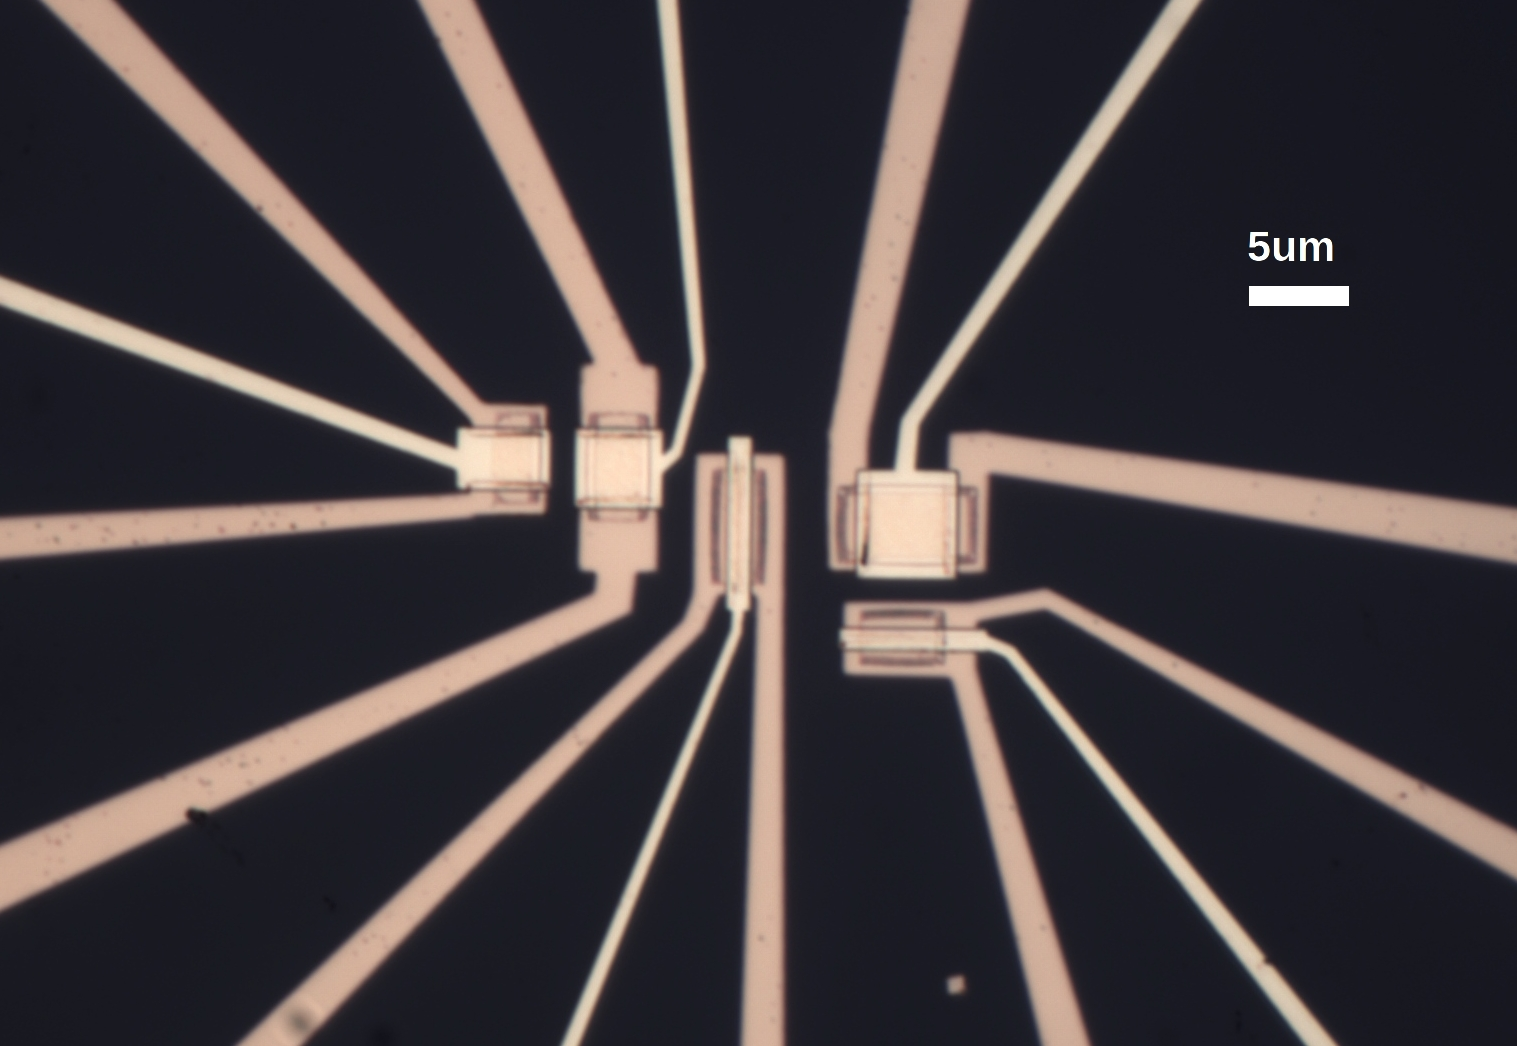
\includegraphics[width=100mm]{figures/magneto/100x_crop.jpg}
\caption{Microscope image of the graphene device used in this chapter. Multiple devices of various geometries are made from the same hBN-graphene-hBN stack on an insulating sapphire substrate. The two-terminal device used in this chapter is the second from the left and has a dimension of $4~\mu m\times4~\mu m$. A lithographically defined local top gate is used to control carrier density.}
\label{fig:m_Giorgio}
\end{figure}
The low temperature, two-terminal resistance varies between $0.2$ and $4.3~k\Omega$ by varying the top gate $\pm5~V$, corresponding to a carrier density of $\sim\pm1.6\times 10^{12}cm^{-2}$, as shown in Fig.~\ref{fig:m_R}. The conductivity minimum is attained for a top gate voltage $V_g = -430~mV$ corresponding to an intrinsic electron doping of $1.4\times 10^{11}cm^{-2}$. The FWHM of the resistance is $5\times 10^{10}cm^{-2}$ with a minimum carrier density of $n_{min}\approx 1.2\times 10^{10}cm^{-2}$, where $n_{min}$ is defined in accordance with chapter~\ref{ch:the_Dirac_fluid}.
\begin{figure}
\centering
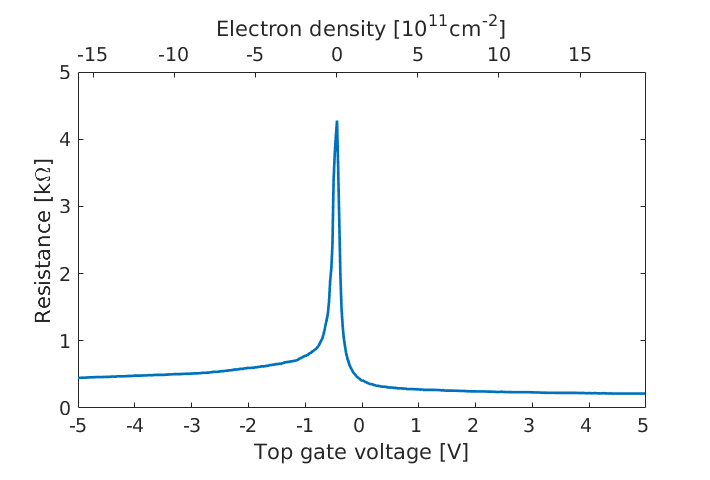
\includegraphics[width=100mm]{figures/magneto/R.png}
\caption{DC resistance of the graphene device at zero magnetic field as a function of carrier density controlled via an electrostatic top gate. Gate capacitance is measured using the integer quantum Hal effect.}
\label{fig:m_R}
\end{figure}

The sample is cooled to $1.7~K$ by a variable temperature, $^4$He vapor cryostat (Appendix~\ref{Appen:Oxford} equipped with a $14~T$ superconducting magnet. The DC two-terminal resistance is measured up to $13~T$ and shown in Fig.~\ref{fig:m_Fan_R}. Integer quantum Hall states are present at fields as low as $0.5~T$ and the $\nu=1$ symmetry broken state appears at high field.
\begin{figure}
\centering
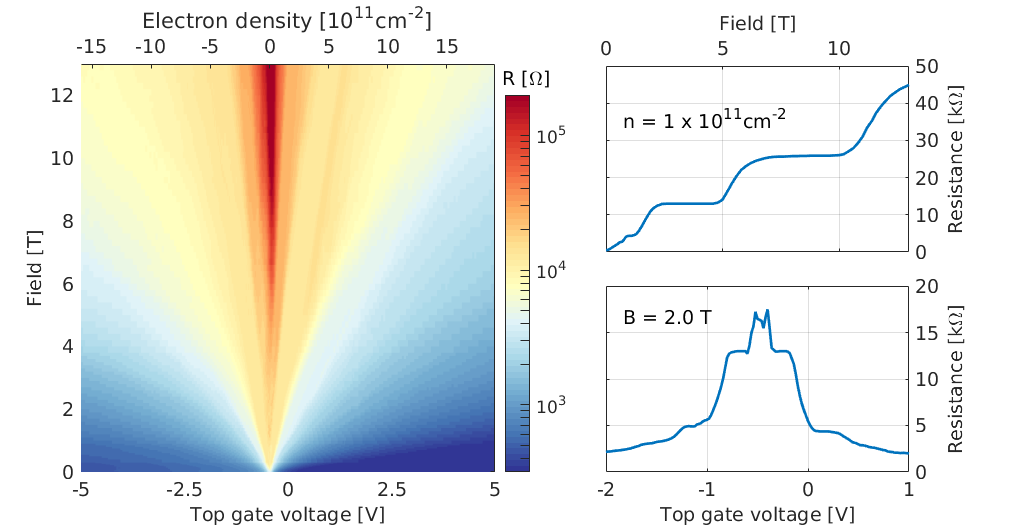
\includegraphics[width=\textwidth]{figures/magneto/Fan_R_cuts.png}
\caption{Two-terminal DC resistance of a monolayer graphene device at $1.7~K$. (\textbf{left}) Resistance is shown on a log scale as a function of carrier density and perpendicular magnetic field strength. (\textbf{top right}) and (\textbf{bottom right}) show cuts at constant density and field, respectively.}
\label{fig:m_Fan_R}
\end{figure}
By analyzing the resistance values of the quantum Hall plateaus, the contact resistance is estimated to vary between $50$ and $170~\Omega$ as a function of density at $1.7~K$. Low contact resistance is vital to Johnson noise thermometry as any dissipation that occurs outside of the sample will lead to unwanted Johnson noise which can degrade the measurement. Using these estimates for the contact resistance, we can estimate the zero field conductivity and thus the Drude mobility and elastic mean free path which vary between $0.2-2\times 10^5~cm^2/Vs$ and $200-650~nm$, respectively, as a function of density, as shown in Fig.~\ref{fig:m_mobility}.
\begin{figure}
\centering
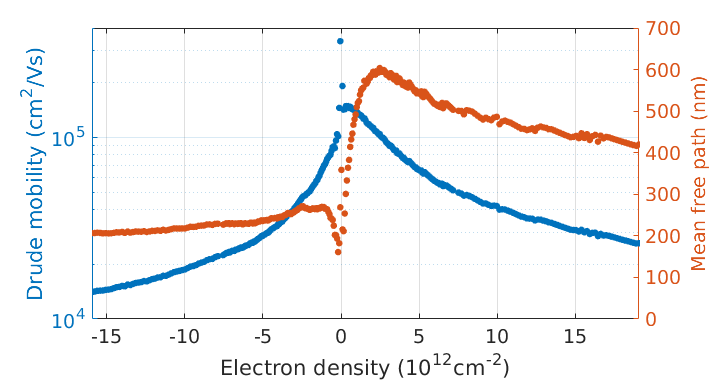
\includegraphics[width=100mm]{figures/magneto/mobility_mfp_1K.png}
\caption{Estimated Drude mobility and elastic mean free path of the graphene device used in this chapter as a function of electron density at $1.7~K$. Estimates are made from the two-terminal conductance at zero magnetic field assuming a contact resistance estimated from the resistance of the integer quantum Hall plateaus. The Drude estimation breaks down near the charge neutrality point where the carrier density is not simply given by the charge density divided by the electron charge}
\label{fig:m_mobility}
\end{figure}

\section{Electrical noise in high fields}
\newthought{Varying by over two orders of magnitude}, the DC resistance of the graphene device must be impedance matched using a wide dynamic range matching network. As described in detail in section~\ref{section:matching}, an on chip, two-stage LC tank circuit in a low-pass configuration is used to transform the sample impedance to near $50~\Omega$. To meet the strict requirements of multi-stage matching, the device was built on an insulating sapphire substrate and surface mount inductors and capacitors were directly soldered to a coplanar waveguide. All inductive elements were air-core as to be magnetic field insensitive and used gold leads which facilitated the direct connection of the graphene sample via wirebond, as shown in Fig.~\ref{fig:m_matching}.
\begin{figure}
\centering
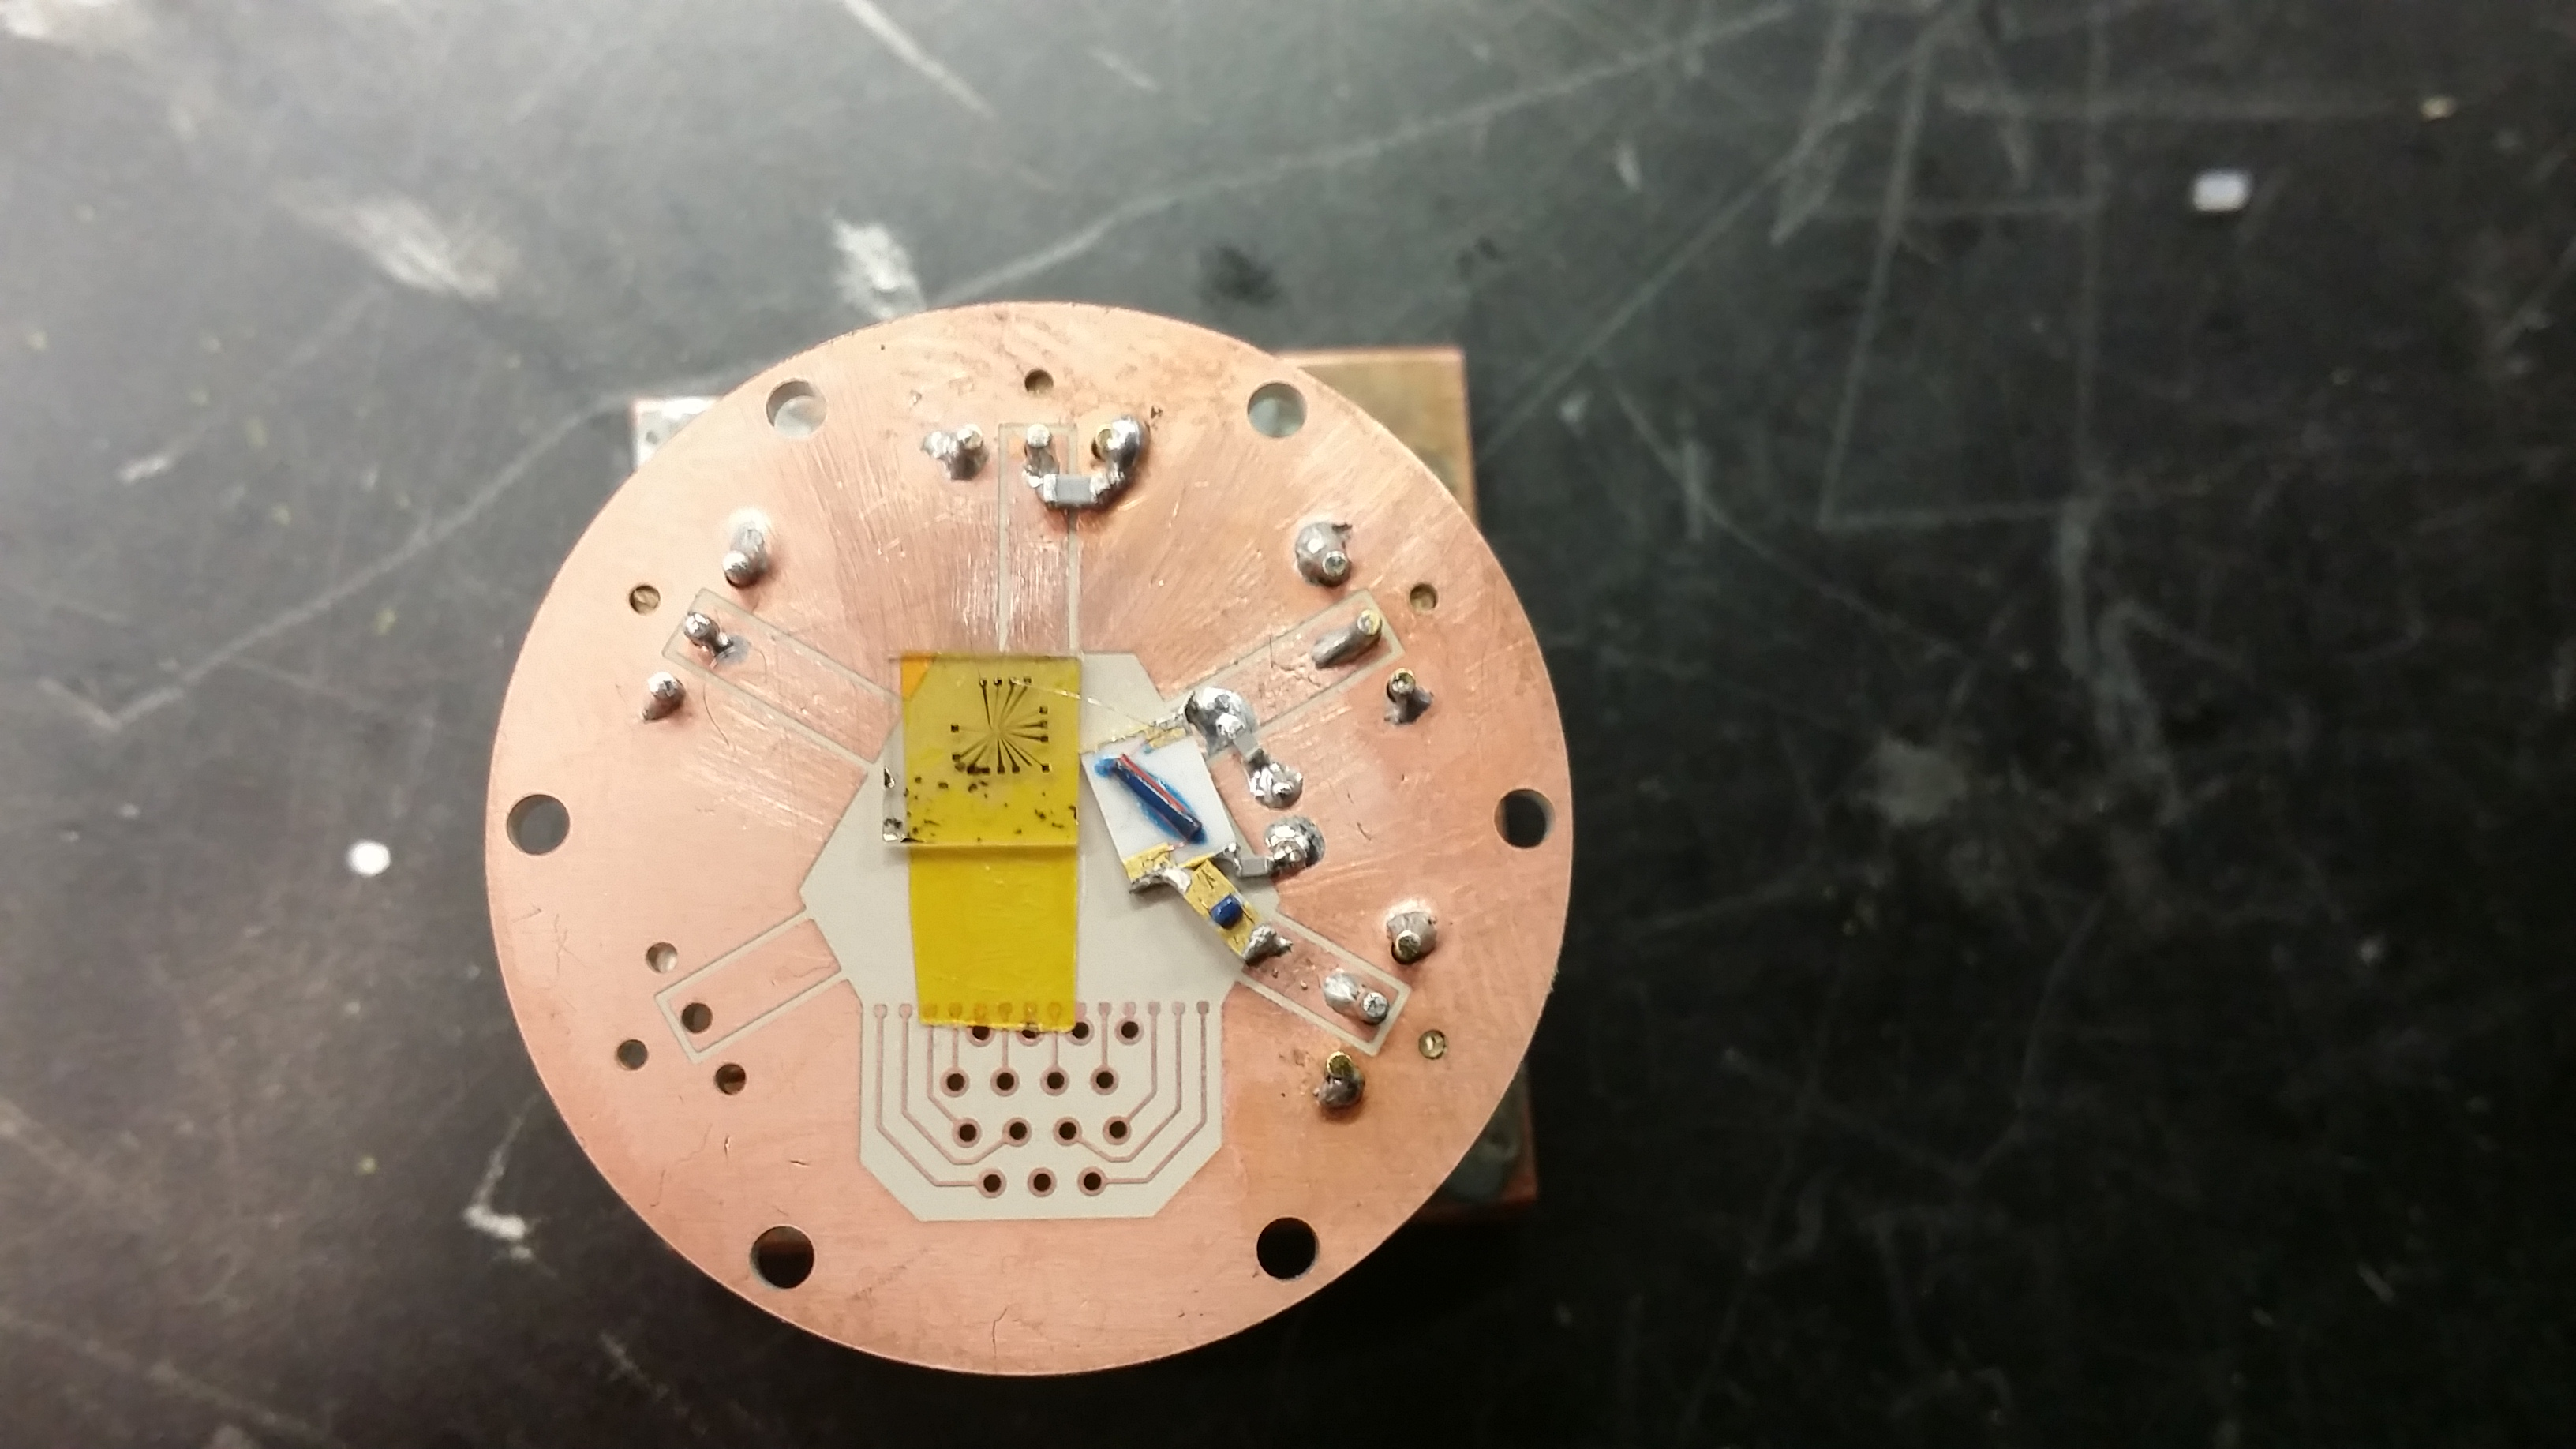
\includegraphics[width=100mm]{figures/magneto/picture_matching_ceramic.jpg}
\caption{Custom sample package used to measure graphene thermal conductance in high magnetic fields. The graphene device is placed on an insulating sapphire substrate which is mounted to the sample package using double-sided Kapton tape. The sample is then wire bonded directly to an air-core surface mount inductor which is part of a two-stage LC tank circuit used to impedance match the high resistance device. The output of the network is soldered directly to a coplanar waveguide which terminates in a high frequency SMP connector. An RF shield then encloses the the device which can be loaded into a cryostat.}
\label{fig:m_matching}
\end{figure}

A vector network analyzer (VNA) can be used to test the high frequency coupling to the device. As the sample resistance changes, different regions of the noise spectra are efficiently coupled into the measurement circuit, as shown in Fig.~\ref{fig:m_S11}. At a DC resistance of $1~k\Omega$ the noise bandwidth of the matching network is ${\sim}150~MHz$ and ${>}3~dB$ coupling continues for resistances above $100~k\Omega$.
\begin{figure}
\centering
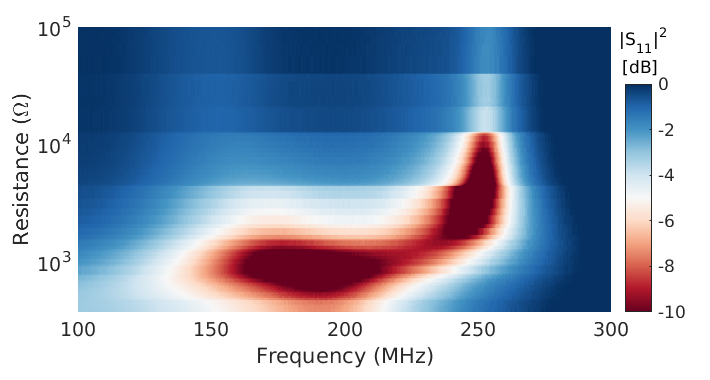
\includegraphics[width=100mm]{figures/magneto/S11_plot.png}
\caption{Reflection coefficient as a function of frequency and graphene DC resistance. The two-stage LC matching circuit is designed to couple a wide dynamic range of resistances allowing the continual measurement of graphene from zero magnetic field to quantum Hall states. When optimally matched at $R\approx~1k\Omega$, the circuit has a noise bandwidth of ${\sim}150~MHz$. As detailed in section~\ref{section:matching}, the high frequency solution of the two-stage network is intentionally moved to a higher resistance creating a wider dynamic range.
}
\label{fig:m_S11}
\end{figure}
Quantifying the coupling in terms of a noise measurement for a circuit as detailed in section~\ref{section:autocorrelation}, we can write the measured output voltage as
\begin{equation}\label{eq:Vout_G_Tn}
V_{out} = \mathcal{G}(\Gamma)(T+T_n(\Gamma)).
\end{equation}
Calibration as outlined in section~\ref{section:calibration} yields $\mathcal{G}(\Gamma)$ and $T_n(\Gamma)$ which are plotted as a function of the DC resistance in Fig.~\ref{fig:m_G_Tn}. We find the calibration parameters to depend only upon the graphene DC resistance and not upon temperature or magnetic field, indicating the matching network is stable over the parameter range of our measurement.
\begin{figure}
\centering
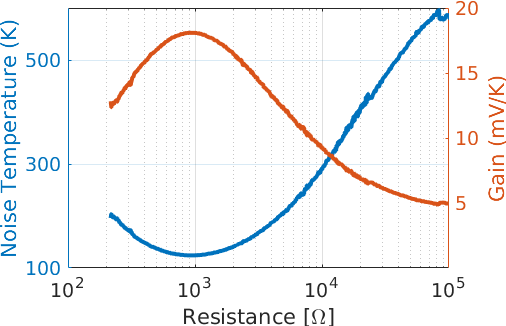
\includegraphics[width=80mm]{figures/magneto/G_Tn.png}
\caption{Generalize gain and noise temperature, as defined in section~\ref{section:system_noise_temperature} and Eqn.~\ref{eq:Vout_G_Tn}, for the graphene device and matching network shown above. Gain is maximize, and noise temperature is minimized when the device is optimally matched at $1~k\Omega$. This data is collected by varying the carrier density of graphene at three different magnetic field values, $0$, $1$, and $13~T$. All data collapses onto the same line indicating the matching circuit is field insensitive and depends only upon the graphene DC resistance.}
\label{fig:m_G_Tn}
\end{figure}
With the device matched and the circuit calibrated, we can measure the total output noise from the sample (Fig.~\ref{fig:m_VNdc}). During the course of an experiment it is common for the background noise $T_n$ to fluctuate on a long time scale (e.g. hours); thus to reach the desired sensitivity it is necessary to perform differential measurements, as described in chapter~\ref{ch:thermal_conductance_via_electrical_noise}, by sinusoidally varying the a Joule heating current and measuring the cosinusoidal electronic temperature rise with a lock-in amplifier.
\begin{figure}
\centering
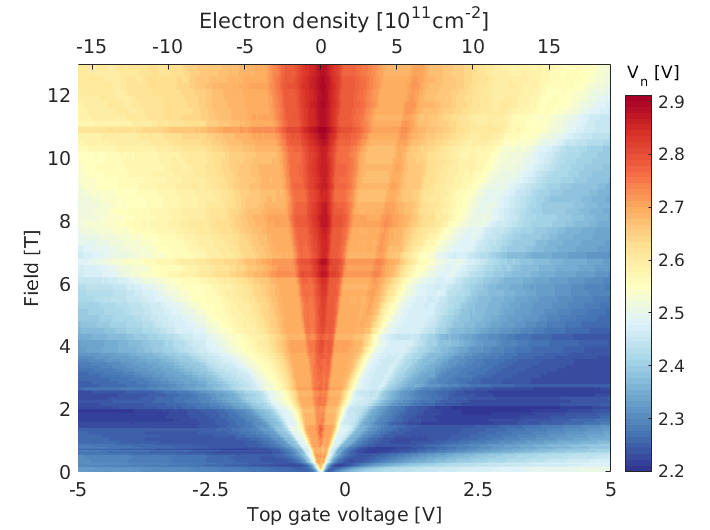
\includegraphics[width=100mm]{figures/magneto/Fan_VNdc.png}
\caption{DC voltage proportional to the total noise emitted into the measurement bandwidth, as defined by Eqn.~\ref{eq:Vout_G_Tn}, from a graphene device as a function of carrier density and magnetic field at $1.7~K$. Horizontal streaks appear in the data as the system noise temperature fluctuates over the course of the experiment illustrating the need for the differential measurements performed in section~\ref{section:magneto-thermal_conductance}.}
\label{fig:m_VNdc}
\end{figure}

\section{Magneto-thermal conductance}
\label{section:magneto-thermal_conductance}
\newthought{While injecting heat into the electronic system}, the steady state temperature rise provides information on how efficiently the system transports thermal energy to the bath. Applying the methodology of chapter~\ref{ch:thermal_conductance_via_electrical_noise}, a differential heating current applies a peak power of $P_0$ to the graphene device and the peak-to-peak differential Johnson noise temperature $\DTJN$ is measured\footnote{Calibration of these differential measurements only requires the use of generalized gain, $\mathcal{G}$. Any fluctuations in the background noise are averaged out and $T_n$ is only important in that it determines how long you must average to reach the desired precision.}. When the device's thermal conductance is large, $\DTJN$ is reduced, while an enhancement of $\DTJN$ signifies a reduction of the thermal conductance. Fig.~\ref{fig:m_DT} shows the differential (quasi-steady state) electronic temperature rise of a square, two-terminal graphene device (described in section~\ref{section:Giorgio}) for a heating power $P_0 = 0.4~n\Watt$. Much of the qualitative heating behavior can be understood via the Wiedemann-Franz law; at low field and high density $\DTJN$ is found to be small, as the electrical conductivity (and therefore the thermal conductivity) is large, while at higher fields, $\DTJN$ is larger due to magnetoresistance affecting the thermal conductivity. At lower density, we find quantum oscillation in the thermal signal and a drastic reduction of $\DTJN$ in quantum Hall states.
\begin{figure}
\centering
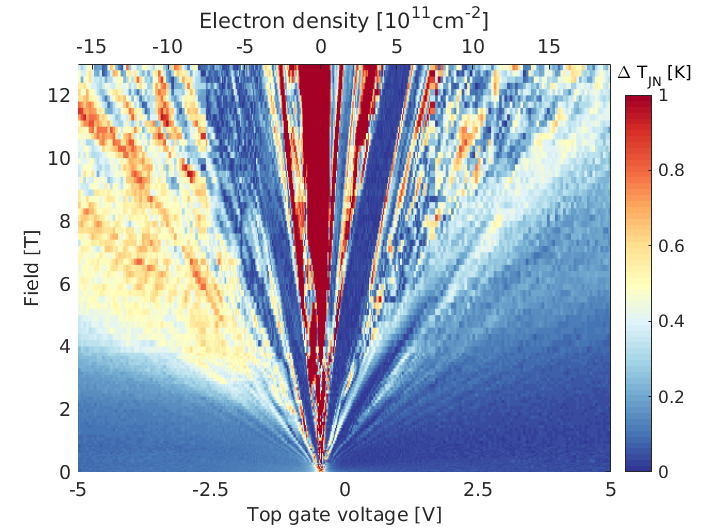
\includegraphics[width=100mm]{figures/magneto/Fan_DT.png}
\caption{Differential Johnson noise temperature rise of a graphene device in response to a differential heating power of $0.4~nW$ as a function of carrier density and magnetic field at $T_b=1.7~K$. At low field and high density, the electronic thermal conductivity is high in accordance with the Wiedemann-Franz law resulting in a small temperature rise. As the field increases, so too does the electrical resistance and thus the thermal resistance and the steady state temperature rise. However, the appearance of quantum effects results in a drastic reduction of $\DTJN$ due to the  ballistic nature of the conduction channel.}
\label{fig:m_DT}
\end{figure}

To analyze this quantitatively, we can define a thermal resistance ($R_{th}$) as the inverse of the thermal conductance defined in chapter~\ref{ch:thermal_conductance_via_electrical_noise},
\begin{equation}
R_{th} \equiv \frac{\DTJN}{P_0}
\end{equation}
Its important to note that $R_{th}$ is not the traditional thermal resistance, which describes the total
heat current flowing through a material in response to a spatial temperature gradient; it is instead
a generalized thermal resistance describing the heat power transferred between the electronic
system and the bath under Joule heating. For a diffusive system\footnote{Here a diffusive system is defined as one where the elastic mean free path of charge carriers is smaller than all other relevant length scales in the problem} dominated by Wiedemann-Franz electronic cooling, the thermal resistance in the linear response regime is given by:
\begin{equation}\label{eq:Rth}
R_{th} = \frac{R}{12\sL~T_b}
\end{equation}
where $\sL$ is the Lorenz ratio and $T_b$ is the bath temperature. Eqn.~\ref{eq:Rth} is derived in section~\ref{section:beta} and holds under the following assumptions:
\begin{enumerate}
\item Heat conduction is provided entirely by electron diffusion of the form $\hat\kappa \propto \hat\sigma$, where the constant of proportionality is defined as $\sL T_b$ by convention
\item The transport coefficients are spatially uniform
\item The device has only two electrical terminals which serve as thermal reservoirs and sources of Joule heating current
\item The elastic mean free path of the charge carriers is shorter than all other relevant length scales in the system
\end{enumerate}
\begin{figure}
\centering
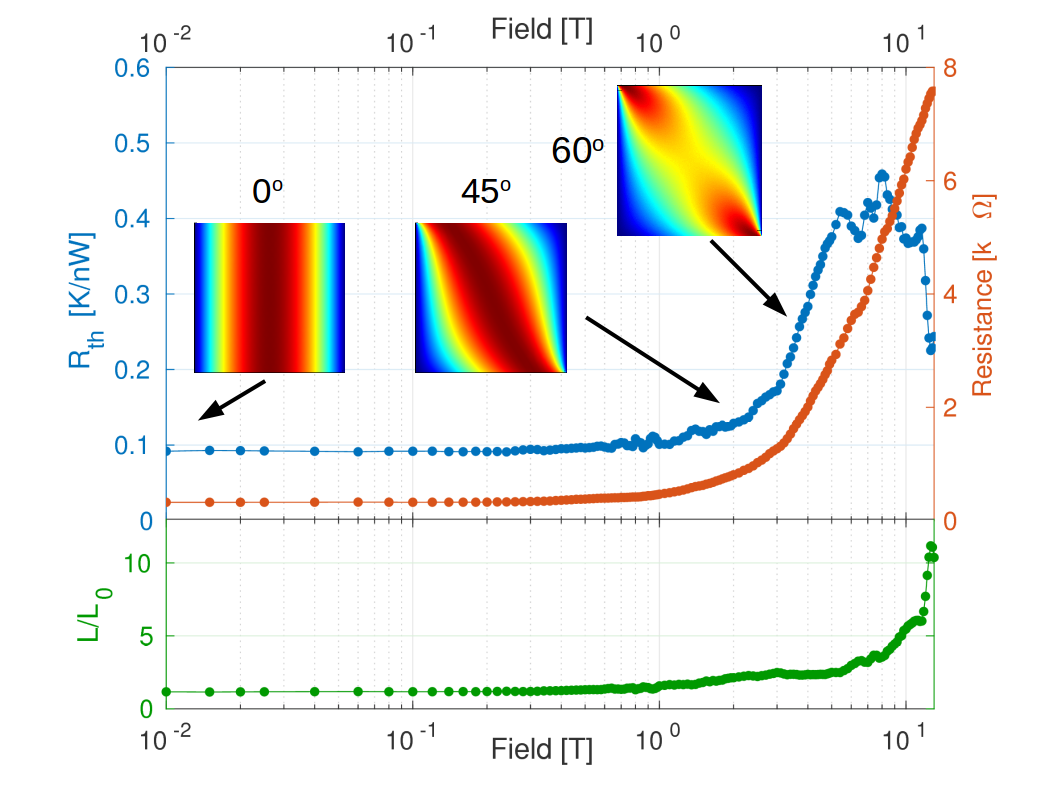
\includegraphics[width=100mm]{figures/magneto/High_density.png}
\caption{(\textbf{upper}) Comparison of the thermal resistance $R_{th}\equiv \DTJN/P_0$ (blue) and the electrical resistance $R$ (red) for monolayer graphene hole doped away from the charge neutrality point ($n\approx-1.6\times10^{12}cm^{-2}$). (\textbf{Insets}) show the expected classical Hall temperature profiles for select Hall angles from finite element simulation~\cite{noauthor_comsol_2017} under the assumption of the WFL. (\textbf{lower}) The measured Lorenz ratio $\sL \equiv (R/R_{th})(1/12T_b)$ normalized to the Sommerfeld value. For magnetic fields below a few Tesla, $R_{th}$ tracks $R$, but at high field, the behavior of $R_{th}$ deviates sharply from that of $R$.}
\label{fig:m_high_density}
\end{figure}

Fig.~\ref{fig:m_high_density} compares $R$ and $R_{th}$ for graphene with a large carrier density ($n\approx -1.6\times10^{12}cm^{-2}$) as a function of magnetic field strength at $10~K$. For fields up to a few Tesla, we find that, while $R_{th}$ qualitatively tracks the field dependence of $R$, the measured Lorenz ratio, $\sL\equiv \frac{1}{12~T_b} (R/R_{th})$, has a small field dependence, even in the so-called ``classical" regime, in stark contrast to the predictions of Eqns.~\ref{eq:Rth} and \ref{eq:WF_gen}. In high field, where landau quantization becomes relevant, the behavior of $R_{th}$ begins to significantly deviate from that of $R$, eventually decreasing with field and tending towards zero. 
\begin{figure}
\centering
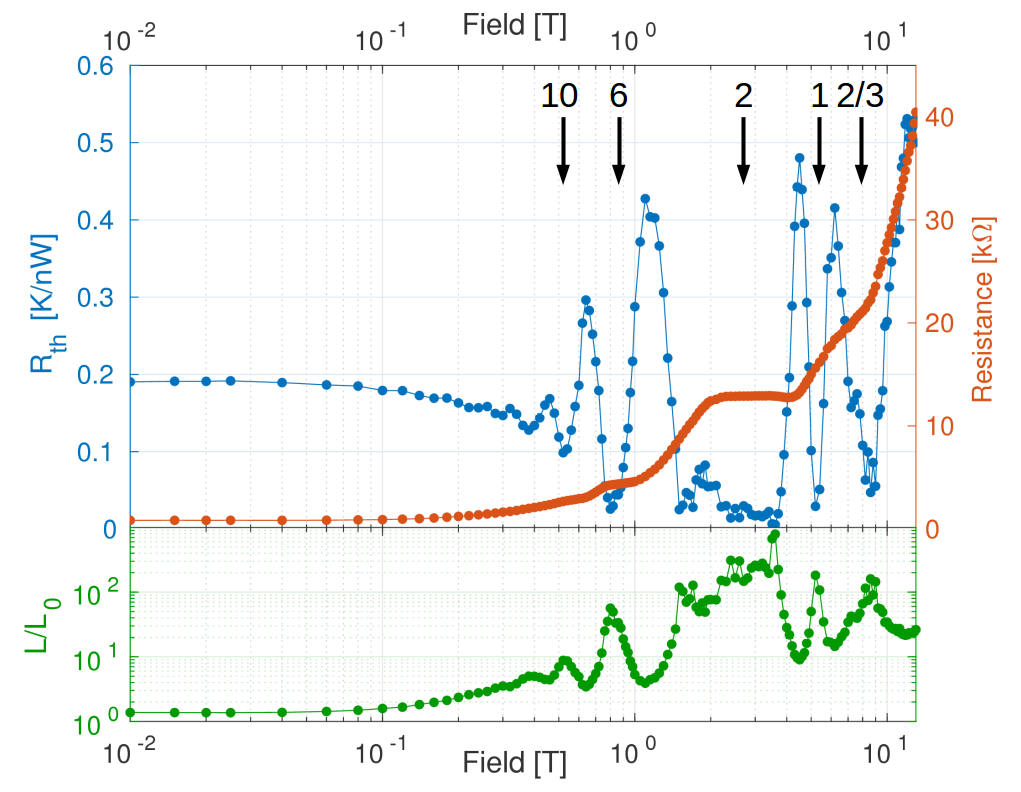
\includegraphics[width=100mm]{figures/magneto/low_density.png}
\caption{(\textbf{upper}) Comparison of the thermal resistance $R_{th}\equiv \DTJN/P_0$ (blue) and the electrical resistance $R$ (red) for monolayer graphene with a carrier (hole) density of $n\approx-1.2\times10^{11}cm^{-2}$. At low field, $R$ increases while $R_{th}$ decreases with quantum oscillations appearing in the thermal data around $0.3~T$. In the $\nu=2$ quantum Hall state, the electrical data shown a plateau at the expected $\frac{1}{2} h/e^2$ while the thermal resistance drops close to zero. At the magnetic field strength corresponding to other filling fractions, $\nu=10$, $6$, $1$, and $2/3$, the thermal signal shows a similar drop toward zero even though the electrical plateaus are not present. (\textbf{lower}) The measured Lorenz ratio $\sL \equiv (R/R_{th})(1/12T_b)$ normalized to the Sommerfeld value.}
\label{fig:m_low_density}
\end{figure}
At low density this behavior is even more pronounced as quantum effects enter as low as $0.5~T$. Fig.~\ref{fig:m_low_density} shows similar measurements to Fig.~\ref{fig:m_high_density} for a lower carrier density of $n\approx-1.2\times10^{11}cm^{-2}$. Unlike the high density data shown in Fig.~\ref{fig:m_high_density}, at low density, $R_{th}$ decreases with magnetic field for low fields even though $R$ increases. For all densities $\sL$ monotonically increases with field until quantum oscillations are seen. At fields and densities where the electrical data shows well developed plateaus, the thermal signal drops to near zero and the measured $\sL$ diverges as a result of the ballistic nature of quantum Hall states. In fact, this combination of Johnson noise thermometry and Joule heating is particularly suited to the detection of quantum modulations of the density of states; this is readily seen in Fig.\ref{fig:m_low_density} where, although not fully developed electrically, the thermal signal shows several more integer states, including the symmetry broken state $\nu=1$, and the fractional state $\nu = 2/3$. The sensitivity of this technique to quantum effects results from its intimate connection to changes in entropy and carrier thermalization length. Fig.~\ref{fig:m_L} shows the entire thermal fan diagram at $T_b=1.7~K$.
\begin{figure}
\centering
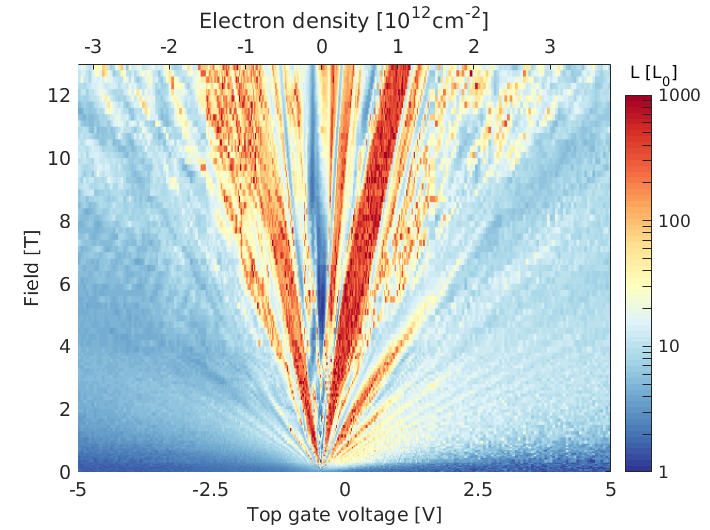
\includegraphics[width=100mm]{figures/magneto/Fan_L.png}
\caption{The measured Lorenz ratio $\sL \equiv (R/R_{th})(1/12T_b)$ of a square graphene device normalized to the Sommerfeld value as a function of carrier density and magnetic field at $T_b=1.7~K$. Color axis shown on a log scale. Quantum Hall states appear as lines of large Lorenz number}
\label{fig:m_L}
\end{figure}

\section{Cyclotron radius}
\newthought{Given the apparent violation} of Eqn.~\ref{eq:Rth} at finite magnetic field, it stands to reason that one of the four assumptions listed above must be violated in graphene. The most obvious of which is the assumption that the elastic mean free path is shorter than all other relevant length scales. In the presence of a magnetic field, electrons in two-dimensional conductors travel along cyclotron orbits of radius 
\begin{equation}
r_c=\frac{m^*v_F}{e~B}
\end{equation}
where $v_F$ is the Fermi velocity and $m^*$ is dynamical mass of the charge carrier. Unlike traditional conductors with parabolic dispersions, the dynamical mass graphene is a function of the Fermi energy ($E_F$) and given by the relativistic form 
\begin{align}
m^* &= E_F/v_F^2 \\
 &= \hbar\sqrt{\pi n}/v_F
\end{align}
thus the cyclotron radius can be written as a function of carrier density and magnetic field, as:
\begin{align}
r_c &= \frac{\hbar\sqrt{\pi n}}{e~B} \\
 &= l_B^2\sqrt{\pi n}
\end{align}
where $l_B = \sqrt{\hbar/eB}$ is the magnetic length. 

\begin{figure}
\centering
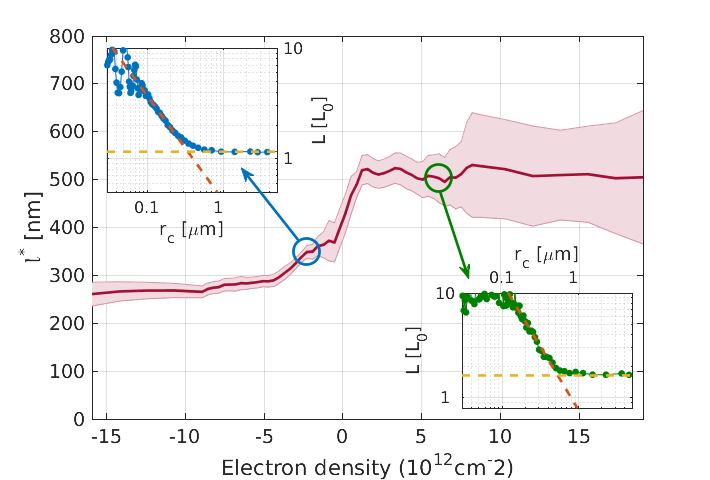
\includegraphics[width=100mm]{figures/magneto/r_cyc.png}
\caption{Characteristic cyclotron radius $l^*(n)$ at which $\sL$ begins to deviate from $\sL_0$. Large cyclotron radius corresponds to small magnetic field. (\textbf{insets}) plot two representative examples of how $l^*$ is extracted; a linear fit to the log of $\sL$ vs cyclotron radius ($r_c$) is extrapolate to the constant, low field value $\sL(B\approx0)$. Red shaded region represents $50\%$ convince intervals of the fits. These values can be directly compared to the quasiparticle elastic mean free path estimated by the zero field conductance in Fig.~\ref{fig:m_mobility}.}
\label{fig:m_cyc}
\end{figure}
As we increase magnetic field for a fixed carrier density, we can quantitatively define a characteristic cyclotron radius ($l^*$) at which $\sL$ begins to deviate from $/sL_0$ by extrapolating a linear fit of the log of $\sL(r_c)$ to the constant low field value $\sL(B\approx0)$. The insets of Fig.~\ref{fig:m_cyc} show two representative examples of this procedure. $l^*(n)$ is the relevant magnetic length at which we see violations of eqn.~\ref{eq:Rth} for a given density. The main panel of Fig.~\ref{fig:m_cyc} plots $l^*$ as a function of electron density. The values found should be quantitatively compared to the elastic mean free path of the charge carriers which is estimated from the zero field conductance in Fig.~\ref{fig:m_mobility}. Essentially, the mean free path imposes a length cutoff for variations of the local temperature --- i.e the temperature cannot equilibrate at scales shorter than the mean-free path, since over these length scales electrons move ballistically. The strong agreement between the data in Figs.~\ref{fig:m_cyc} and \ref{fig:m_mobility} (rms normalized error of $23\%$) is evidence that the deviations of $\sL$ from $\sL_0$ are due to relevant dynamics occurring on a length scale where electrons are ballistic. This is taken to an extreme in the limit of quantum Hall where conduction occurs only on ballistic edge channels and hence the measured Lorenz ratio diverges.

